\documentclass[12pt,a4paper]{article}

% ── Paquetes ──────────────────────────────────────────────────
\usepackage[utf8]{inputenc}
\usepackage[T1]{fontenc}
\usepackage[spanish,mexico]{babel}
\usepackage{geometry}
\usepackage{graphicx}
\usepackage[table]{xcolor}
\usepackage{booktabs}
\usepackage{longtable}
\usepackage{array}
\usepackage{tabularx}
\usepackage{fancyhdr}
\usepackage{titlesec}
\usepackage{setspace}
\usepackage{hyperref}
\usepackage{listings}

% ── Geometría ─────────────────────────────────────────────────
\geometry{margin=2.5cm}
\setstretch{1.2}
\setlength{\headheight}{14pt}

% ── Colores ───────────────────────────────────────────────────
\definecolor{verdeAbejaNet}{RGB}{76,175,80}
\definecolor{azulEncabezado}{RGB}{33,47,61}
\definecolor{grisCelda}{RGB}{245,245,245}
\definecolor{rojoAlerta}{RGB}{198,40,40}
\definecolor{codeBg}{RGB}{248,248,248}
\definecolor{codeFrame}{RGB}{200,200,200}

% ── Hiperenlaces ──────────────────────────────────────────────
\hypersetup{
  colorlinks=true,
  linkcolor=azulEncabezado,
  urlcolor=verdeAbejaNet,
  pdftitle={Reporte Practica 1 -- AbejaNet},
  pdfauthor={Marco Antonio Gomez Olvera},
}

% ── Encabezado y pie ──────────────────────────────────────────
\pagestyle{fancy}
\fancyhf{}
\fancyhead[L]{\small\textit{AbejaNet -- Preprocesamiento de Datos}}
\fancyhead[R]{\small\textit{Extracci\'on de Conocimiento en BD}}
\fancyfoot[C]{\thepage}
\renewcommand{\headrulewidth}{0.4pt}

% ── T\'itulos ─────────────────────────────────────────────────
\titleformat{\section}{\Large\bfseries\color{azulEncabezado}}{\thesection}{1em}{}
\titleformat{\subsection}{\large\bfseries\color{azulEncabezado}}{\thesubsection}{1em}{}
\titleformat{\subsubsection}{\normalsize\bfseries\color{azulEncabezado}}{\thesubsubsection}{1em}{}

% ── C\'odigo ──────────────────────────────────────────────────
\lstset{
  backgroundcolor=\color{codeBg},
  frame=single, rulecolor=\color{codeFrame},
  basicstyle=\ttfamily\footnotesize,
  breaklines=true,
  numbers=none,
  keepspaces=true,
}

% ── Comandos ──────────────────────────────────────────────────
\newcommand{\badge}[2]{\colorbox{#1}{\color{white}\textbf{\small #2}}}

% ══════════════════════════════════════════════════════════════
\begin{document}
% ══════════════════════════════════════════════════════════════

\begin{titlepage}
  \begin{spacing}{1}
  \centering
  \vspace*{0.3cm}

  
\includegraphics[width=3.8cm]{images/logo_uteq.png}\\[0.5cm]

  {\color{verdeAbejaNet}\rule{\textwidth}{2.5pt}}\\[0.5cm]

  {\LARGE\bfseries Evaluaci\'on Unidad I}\\[0.25cm]
  {\Large\bfseries Preprocesamiento y Almacenamiento de Datos}\\[0.3cm]
  {\large\color{azulEncabezado}\bfseries AbejaNet Revival --- Sistema IoT de Monitoreo de Colmenas}\\[0.6cm]

  {\color{verdeAbejaNet}\rule{\textwidth}{1pt}}\\[0.4cm]

  {\large\textbf{Asignatura:}}\\
  Extracci\'on de Conocimiento en Bases de Datos\\[0.3cm]
  {\large\textbf{Carrera:}}\\
  Ingenier\'ia en Desarrollo y Gesti\'on de Software\\[0.3cm]
  {\large\textbf{Grupo:}} IDGS 16
  \hspace{2cm}
  {\large\textbf{Periodo:}} Mayo -- Agosto 2026\\[0.5cm]

  {\color{verdeAbejaNet}\rule{\textwidth}{1pt}}\\[0.4cm]

  {\large\textbf{Equipo de Trabajo}}\\[0.3cm]

  \begin{tabular}{ll}
    \textbf{Marco Antonio G\'omez Olvera}  & Programador de la Aplicaci\'on M\'ovil \\[0.2em]
    \textbf{Orlando Rubio Cabrera}          & Encargado de IoT \\[0.2em]
    \textbf{Sandra Zo\'e Cabrera Vel\'azquez} & Encargada de Documentaci\'on \\[0.2em]
    \textbf{Israel G\'omez Bonilla}         & Desarrollador de la Aplicaci\'on Web \\
  \end{tabular}\\[0.6cm]

  {\color{verdeAbejaNet}\rule{\textwidth}{1pt}}\\[0.4cm]

  {\large\textbf{Unidad Tecnol\'ogica de Quer\'etaro (UTEQ)}}\\[0.2cm]
  {\normalsize Quer\'etaro, junio de 2026}

  \vfill
  \end{spacing}
\end{titlepage}


\tableofcontents
\newpage

\section{Contexto del Caso de Estudio}

\textbf{AbejaNet Revival} es una plataforma IoT para monitoreo en tiempo real de colmenas
de abejas (\textit{Apis mellifera}). El sistema integra sensores ESP32 instalados en las
colmenas para recopilar variables ambientales (temperatura, humedad, peso, decibelios y
lluvia), un backend Node.js/Express con base de datos PostgreSQL, una aplicaci\'on m\'ovil
React Native/Expo y un panel web de administraci\'on.

La tabla \texttt{lecturas\_ambientales} de la base de datos operacional constituye la
fuente principal de datos de esta evaluaci\'on. Dado que el servidor de producci\'on
(Render) no estaba activo durante el periodo de desarrollo, los datos se generaron de forma
sint\'etica con el script \texttt{00\_generar\_datos.py}, replicando la l\'ogica de
simulaci\'on del archivo original \texttt{backend/generate\_mock\_data.js} del proyecto.

\subsection{Arquitectura del Sistema}

\begin{itemize}\setlength{\itemsep}{2pt}
  \item \textbf{Sensores ESP32:} Env\'ian lecturas v\'ia POST \texttt{/api/sensor-data}
        cada 10 minutos con autenticaci\'on por clave API.
  \item \textbf{Backend Node.js/Express:} Recibe, valida y persiste los datos en
        PostgreSQL alojado en Render.
  \item \textbf{Aplicaci\'on m\'ovil:} Consume la API REST con autenticaci\'on JWT,
        mostrando gr\'aficas de tendencias por colmena.
  \item \textbf{Panel web:} Gesti\'on de usuarios, apiarios, colmenas y alertas.
\end{itemize}

\subsection{Colmenas Monitoreadas}

\begin{table}[h!]
  \centering
  \rowcolors{2}{grisCelda}{white}
  \begin{tabular}{llll}
    \toprule
    \textbf{Apiario} & \textbf{Colmena} & \textbf{MAC} & \textbf{Tipo Sensor} \\
    \midrule
    Apiario Principal   & Colmena Alfa Ppal  & AA:BB:CC:11:22:33 & Temperatura/Humedad \\
    Apiario Principal   & Colmena Gamma Ppal & AA:BB:CC:11:22:44 & Multisensor \\
    Apiario Laboratorio & Colmena Beta Lab   & A2:04:2A:B9:C1:D9 & Multisensor \\
    \bottomrule
  \end{tabular}
  \caption{Inventario de colmenas y sensores del sistema AbejaNet}
\end{table}

\newpage

\section{SA --- Evidencia del Saber: Arquitectura del Data Warehouse}

\subsection{Esquema de Data Warehouse --- Estrella (Star Schema)}

Se opt\'o por el \textbf{Esquema en Estrella} debido a que la tabla de hechos
(\texttt{fact\_lecturas\_ambientales}) contiene m\'etricas num\'ericas bien definidas,
las dimensiones tienen cardinalidad estable (Slowly Changing Dimensions tipo 1), y el
modelo ofrece mayor eficiencia en consultas OLAP que el esquema copo de nieve.

\begin{table}[h!]
  \centering
  \caption{Tabla de Hechos: \texttt{fact\_lecturas\_ambientales}}
  \rowcolors{2}{grisCelda}{white}
  \begin{tabularx}{\textwidth}{llX}
    \toprule
    \textbf{Columna} & \textbf{Tipo} & \textbf{Descripci\'on} \\
    \midrule
    \texttt{id\_lectura}  & BIGSERIAL PK  & Clave surrogate autogenerada \\
    \texttt{sk\_sensor}   & INTEGER FK    & $\rightarrow$ \texttt{dim\_sensor} \\
    \texttt{sk\_tiempo}   & INTEGER FK    & $\rightarrow$ \texttt{dim\_tiempo} \\
    \texttt{sk\_colmena}  & INTEGER FK    & $\rightarrow$ \texttt{dim\_colmena} \\
    \texttt{sk\_apiario}  & INTEGER FK    & $\rightarrow$ \texttt{dim\_apiario} \\
    \texttt{temperatura}  & DECIMAL(5,2)  & \textcelsius{} interior de la colmena \\
    \texttt{humedad}      & DECIMAL(5,2)  & \% de humedad relativa \\
    \texttt{peso}         & DECIMAL(6,2)  & kg totales de la colmena (NULL si no aplica) \\
    \texttt{sonido}       & DECIMAL(5,2)  & dB de actividad son\'ora \\
    \texttt{lluvia}       & SMALLINT      & 1~=~lluvia, 0~=~sin lluvia \\
    \texttt{alerta\_temp} & SMALLINT      & 1 si temperatura $>$ 35\textcelsius{} (calculado) \\
    \bottomrule
  \end{tabularx}
\end{table}

\textbf{Granularidad:} una fila representa la lectura de un sensor cada 15 minutos.

\begin{table}[h!]
  \centering
  \caption{Dimensiones del Data Warehouse}
  \rowcolors{2}{grisCelda}{white}
  \begin{tabularx}{\textwidth}{llX}
    \toprule
    \textbf{Dimensi\'on} & \textbf{Clave PK} & \textbf{Atributos principales} \\
    \midrule
    \texttt{dim\_tiempo}  & \texttt{sk\_tiempo}  & fecha\_completa, a\~no, mes, semana, dia\_semana, hora, periodo\_dia, es\_noche, es\_fin\_semana, es\_hora\_activa\_abejas \\
    \texttt{dim\_sensor}  & \texttt{sk\_sensor}  & mac\_address, tipo\_sensor, estado, fecha\_instalacion \\
    \texttt{dim\_colmena} & \texttt{sk\_colmena} & nombre\_colmena, descripcion, fecha\_creacion \\
    \texttt{dim\_apiario} & \texttt{sk\_apiario} & nombre\_apiario, descripcion\_general, coordenadas \\
    \bottomrule
  \end{tabularx}
\end{table}

\subsection{Tipos y Fuentes de Datos}

\begin{table}[h!]
  \centering
  \caption{Inventario de variables por tipo estad\'istico}
  \rowcolors{2}{grisCelda}{white}
  \begin{tabularx}{\textwidth}{lllX}
    \toprule
    \textbf{Variable} & \textbf{Tipo} & \textbf{Escala} & \textbf{Rango / Valores} \\
    \midrule
    \texttt{temperatura}  & Continua    & Raz\'on    & $[0, 45]$ \textcelsius{} \\
    \texttt{humedad}      & Continua    & Raz\'on    & $[40, 95]$ \% \\
    \texttt{peso}         & Continua    & Raz\'on    & $[10, 30]$ kg \\
    \texttt{sonido}       & Continua    & Raz\'on    & $[40, 80]$ dB \\
    \texttt{lluvia}       & Discreta    & Nominal    & $\{0, 1\}$ \\
    \texttt{tipo\_sensor} & Categ\'orica & Nominal   & Temperatura/Humedad, Multisensor \\
    \texttt{estado}       & Categ\'orica & Ordinal   & activo, mantenimiento, inactivo, no\_asignado \\
    \texttt{hora}         & Discreta    & C\'iclica  & $[0, 23]$ \\
    \texttt{dia\_semana}  & Discreta    & Ordinal    & $[0, 6]$ \\
    \texttt{es\_noche}    & Discreta    & Nominal    & $\{0, 1\}$ \\
    \texttt{alerta\_temp} & Discreta    & Nominal    & $\{0, 1\}$ (variable objetivo) \\
    \bottomrule
  \end{tabularx}
\end{table}

\begin{table}[h!]
  \centering
  \caption{Fuentes de datos del proyecto}
  \rowcolors{2}{grisCelda}{white}
  \begin{tabularx}{\textwidth}{llX}
    \toprule
    \textbf{Fuente} & \textbf{Tipo} & \textbf{Descripci\'on} \\
    \midrule
    ESP32 $\rightarrow$ POST \texttt{/api/sensor-data} & Estructurada en tiempo real & Lecturas cada 10 min con cabecera X-API-Key \\
    \texttt{generate\_mock\_data.js} & Sint\'etica estructurada & Simulaci\'on de 30 d\'ias en Node.js \\
    \texttt{00\_generar\_datos.py}   & Sint\'etica estructurada & Dataset de esta pr\'actica con problemas de calidad intencionales \\
    \texttt{abeja\_net\_v4\_postgres.sql} & Relacional & Esquema oficial + datos semilla de la BD \\
    \bottomrule
  \end{tabularx}
\end{table}

\subsection{T\'ecnicas de Limpieza de Datos}

\begin{table}[h!]
  \centering
  \caption{T\'ecnicas de limpieza aplicadas y su justificaci\'on}
  \rowcolors{2}{grisCelda}{white}
  \begin{tabularx}{\textwidth}{lX}
    \toprule
    \textbf{T\'ecnica} & \textbf{Justificaci\'on y Aplicaci\'on} \\
    \midrule
    Forward fill (ffill) por grupo & Variables de serie temporal: el valor m\'as reciente del mismo sensor es la mejor estimaci\'on de un dato faltante. Respeta la autocorrelaci\'on temporal. \\
    Eliminaci\'on de duplicados     & Un sensor no puede tener dos lecturas en el mismo instante (\texttt{sensor\_id + fecha\_registro}). Duplicados exactos eliminados con \texttt{drop\_duplicates}. \\
    Reglas de negocio (outliers)   & Temperatura fuera de $[0, 45]$\textcelsius{} o humedad fuera de $[0, 100]$\% son f\'isicamente imposibles $\rightarrow$ se invalidan como NaN y se reimputan. \\
    Interpolaci\'on lineal (peso)   & El peso de la colmena crece de forma gradual y predecible. La interpolaci\'on lineal es apropiada entre puntos cercanos. \\
    Mapeo de formatos               & \texttt{lluvia} pod\'ia llegar como \texttt{True/False}, \texttt{"si"/"no"} o \texttt{1/0}. Se normaliz\'o todo a entero $\{0, 1\}$. \\
    Eliminaci\'on de hu\'erfanos    & Registros sin \texttt{sensor\_id} no pueden asociarse a ninguna colmena y se eliminan. \\
    \bottomrule
  \end{tabularx}
\end{table}

\subsection{Par\'ametros de Configuraci\'on del Data Warehouse (PostgreSQL local)}

\begin{lstlisting}[language=SQL, caption=Esquema y \'indices de optimizaci\'on para el DW]
CREATE SCHEMA abejanet_dw;

-- Indices principales para JOINs OLAP
CREATE INDEX idx_fact_sk_sensor  ON fact_lecturas_ambientales (sk_sensor);
CREATE INDEX idx_fact_sk_tiempo  ON fact_lecturas_ambientales (sk_tiempo);
CREATE INDEX idx_fact_sk_colmena ON fact_lecturas_ambientales (sk_colmena);
CREATE INDEX idx_dim_tiempo_fecha ON dim_tiempo (fecha_completa);
CREATE INDEX idx_dim_tiempo_hora  ON dim_tiempo (hora, es_noche);

-- postgresql.conf recomendado para analisis local
-- shared_buffers       = 512MB
-- work_mem             = 64MB
-- effective_cache_size = 2GB
-- max_parallel_workers_per_gather = 4
\end{lstlisting}

\subsection{Repositorio T\'ecnico}

El conjunto de datos preprocesado, los scripts y los archivos de log se encuentran
en el repositorio p\'ublico:

\begin{center}
  \url{https://github.com/MarkG777/Evaluacion_BD}
\end{center}

Los archivos entregados son:
\texttt{data/raw/lecturas\_crudas.csv} (datos crudos),
\texttt{data/clean/lecturas\_limpias.csv} (datos limpios) y
\texttt{data/clean/dataset\_final\_features.csv} (dataset optimizado AU).

\newpage

\section{DE --- Evidencia de Desempe\~no: Proceso de Limpieza Paso a Paso}

El script \texttt{02\_de\_limpieza\_pipeline.py} aplica diez transformaciones sobre el
dataset crudo y produce un log completo (\texttt{data/clean/log\_limpieza.txt}) con
evidencia cuantitativa de cada paso.

\subsection{Problemas de Calidad Identificados}

\begin{table}[h!]
  \centering
  \caption{Problemas de calidad presentes en \texttt{lecturas\_crudas.csv}}
  \rowcolors{2}{grisCelda}{white}
  \begin{tabularx}{\textwidth}{lrX}
    \toprule
    \textbf{Problema} & \textbf{Cantidad} & \textbf{T\'ecnica aplicada} \\
    \midrule
    Nulos en \texttt{temperatura}          & 346 (4.06\%)   & Forward fill por sensor \\
    Nulos en \texttt{humedad}              & 438 (4.99\%)   & Forward fill por sensor \\
    Nulos en \texttt{sonido}               & 267 (3.04\%)   & Forward fill por sensor \\
    Outliers temperatura $>$45\textcelsius{} o $<$0\textcelsius{} & 76 & Invalidar $\rightarrow$ NaN $\rightarrow$ reimputar \\
    Outliers humedad $>$100\%              & 67             & Invalidar $\rightarrow$ NaN $\rightarrow$ reimputar \\
    Filas duplicadas (exactas)             & 127            & \texttt{drop\_duplicates()} \\
    Duplicados sensor+timestamp            & 1              & \texttt{drop\_duplicates(subset)} \\
    Formato incorrecto en \texttt{lluvia}  & 351 (4\%)      & Mapeo normalizado a \texttt{int} $\{0,1\}$ \\
    Registros hu\'erfanos sin sensor\_id   & 68             & Eliminaci\'on \\
    \bottomrule
  \end{tabularx}
\end{table}

\subsection{Resultados del Pipeline --- Antes vs.\ Despu\'es}

\begin{table}[h!]
  \centering
  \caption{Evidencia cuantitativa de cada paso del pipeline}
  \rowcolors{2}{grisCelda}{white}
  \begin{tabularx}{\textwidth}{clrrX}
    \toprule
    \textbf{Paso} & \textbf{T\'ecnica} & \textbf{Antes} & \textbf{Despu\'es} & $\Delta$ \\
    \midrule
    0 & Carga del dataset crudo              & ---   & 8\,769 & --- \\
    1 & Correcci\'on de tipos y formatos      & 8\,769 & 8\,769 & 0 filas, 0 nulos \\
    2 & Eliminaci\'on de duplicados           & 8\,769 & 8\,641 & $-128$ filas \\
    3 & Eliminaci\'on de hu\'erfanos          & 8\,641 & 8\,573 & $-68$ filas \\
    4 & Invalidaci\'on de outliers            & 8\,573 & 8\,573 & $+143$ nulos \\
    5 & Imputaci\'on ffill+bfill              & 8\,573 & 8\,573 & $-1\,164$ nulos \\
    6 & Enriquecimiento temporal              & 13 cols & 21 cols & $+8$ features \\
    7 & Validaci\'on final de rangos          & ---   & OK    & Sin errores \\
    \midrule
    \multicolumn{2}{l}{\textbf{Total removidos}} & 8\,769 & \textbf{8\,573} & $-196$ (2.24\%) \\
    \bottomrule
  \end{tabularx}
\end{table}

\subsection{Evidencia Visual --- Paso 1: Correcci\'on de Formatos}

\begin{lstlisting}[caption=Salida real del PASO 1 -- correcci\'on de tipos]
[1a] fecha_registro
     Tipo antes  : object (str)
     Tipo despues: datetime64[us]
     Fechas invalidas (NaT): 0

[1b] lluvia
     Valores antes  : ['False' 'no' 'True' 'si']
     Valores despues: [0 1]
     Tipo despues   : int8

[1c] sensor_id
     Tipo despues: Int64  (NaN conservados: 69)
\end{lstlisting}

\subsection{Evidencia Visual --- Paso 4: Diagn\'ostico de Outliers (IQR)}

\begin{lstlisting}[caption=Salida real del PASO 4 -- deteccion y tratamiento de outliers]
[temperatura (diagnostico IQR)]
  Q1=22.36  Q3=32.14  IQR=9.79
  Limites IQR: [7.68, 46.82]
  Outliers estadisticos: 86 (1.04%)
  -> Regla de negocio: temperatura fuera de [0.0, 45.0] C -> NaN
  -> Outliers invalidados: 76

[humedad (diagnostico IQR)]
  Q1=53.35  Q3=70.67  IQR=17.32
  Limites IQR: [27.37, 96.65]
  Outliers estadisticos: 67 (0.82%)
  -> Regla de negocio: humedad fuera de [0, 100]% -> NaN
  -> Outliers invalidados: 67
\end{lstlisting}

\subsection{Estadísticas Descriptivas Post-limpieza (Paso 7)}

\begin{lstlisting}[caption=Salida real del PASO 7 -- estadisticas descriptivas finales]
         temperatura   humedad      peso    sonido
count       8573.000  8573.000  5710.000  8573.000
mean          27.195    61.955    15.910    57.679
std            5.104     9.157     0.737     8.509
min            0.040    44.270    14.440    44.000
25%           22.380    53.320    15.310    49.440
50%           27.190    62.010    15.910    60.770
75%           32.100    70.520    16.510    65.480
max           35.940    79.580    17.380    70.000

Distribucion por colmena:
  Colmena Alfa Ppal     2863 lecturas
  Colmena Gamma Ppal    2860 lecturas
  Colmena Beta Lab      2850 lecturas

Validaciones de rango superadas: temperatura [0,45] OK | humedad [0,100] OK
Dataset limpio: 8573 filas x 21 columnas
\end{lstlisting}

\subsection{Archivos Generados}

\begin{itemize}\setlength{\itemsep}{2pt}
  \item \texttt{data/raw/lecturas\_crudas.csv} --- 8\,769 filas $\times$ 13 columnas (datos con suciedad intencional)
  \item \texttt{data/clean/lecturas\_limpias.csv} --- 8\,573 filas $\times$ 21 columnas (dataset limpio + features temporales)
  \item \texttt{data/clean/log\_limpieza.txt} --- log completo de ejecuci\'on con evidencia de cada transformaci\'on
\end{itemize}

\newpage

\section{AU --- Evidencia Aut\'onoma: Selecci\'on de Caracter\'isticas Avanzada}

\subsection{Variable Objetivo}

\textbf{Target:} \texttt{alerta\_temperatura} = 1 si temperatura $>$ 35\textcelsius{}

Owens (1971) y Seeley (1985) documentan que por encima de 35\textcelsius{} las abejas de
ventilaci\'on (\textit{fanners}) se activan masivamente, lo que se manifiesta en un
incremento del nivel sonoro, descenso de humedad interior y potencial p\'erdida de peso
por enjambre. Distribuci\'on: 8\,364 negativos (97.6\%) y 209 positivos (2.4\%).

\subsection{M\'etodo 1 --- Correlaci\'on de Pearson}

La correlaci\'on de Pearson mide la relaci\'on lineal entre cada variable num\'erica y el
target. Umbral de corte: $|r| \geq 0.02$. Ninguna feature fue descartada por este
m\'etodo --- todas presentan alguna relaci\'on lineal con \texttt{alerta\_temperatura}.

\begin{figure}[h!]
  \centering
  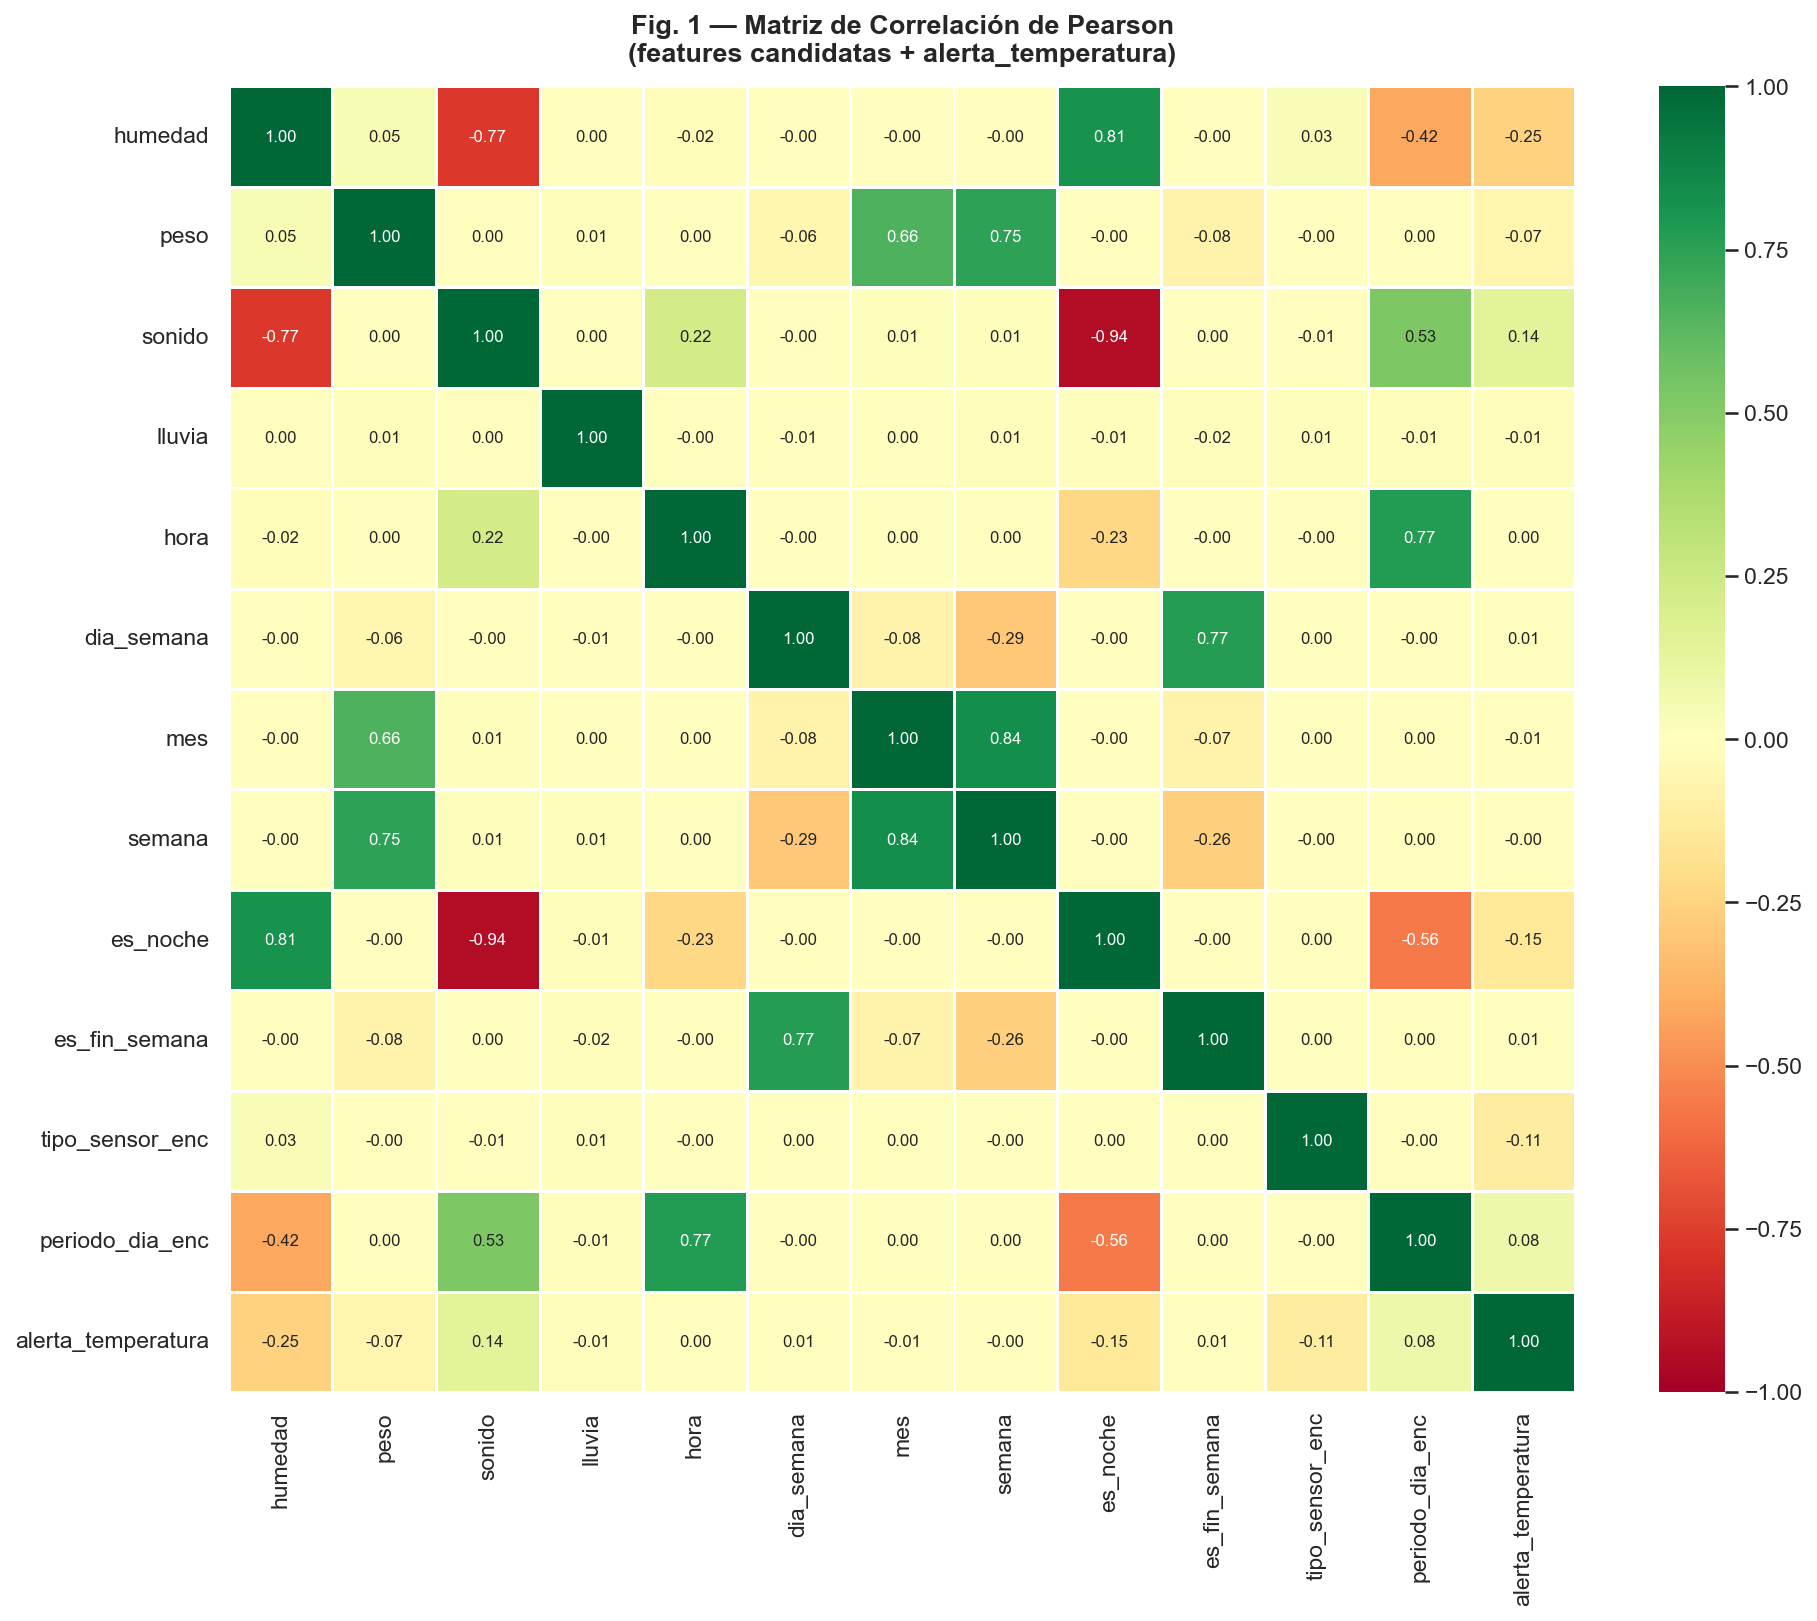
\includegraphics[width=\textwidth]{figures/fig1_heatmap_correlacion.png}
  \caption{Matriz completa de correlaci\'on de Pearson (features candidatas + target)}
\end{figure}

\begin{figure}[h!]
  \centering
  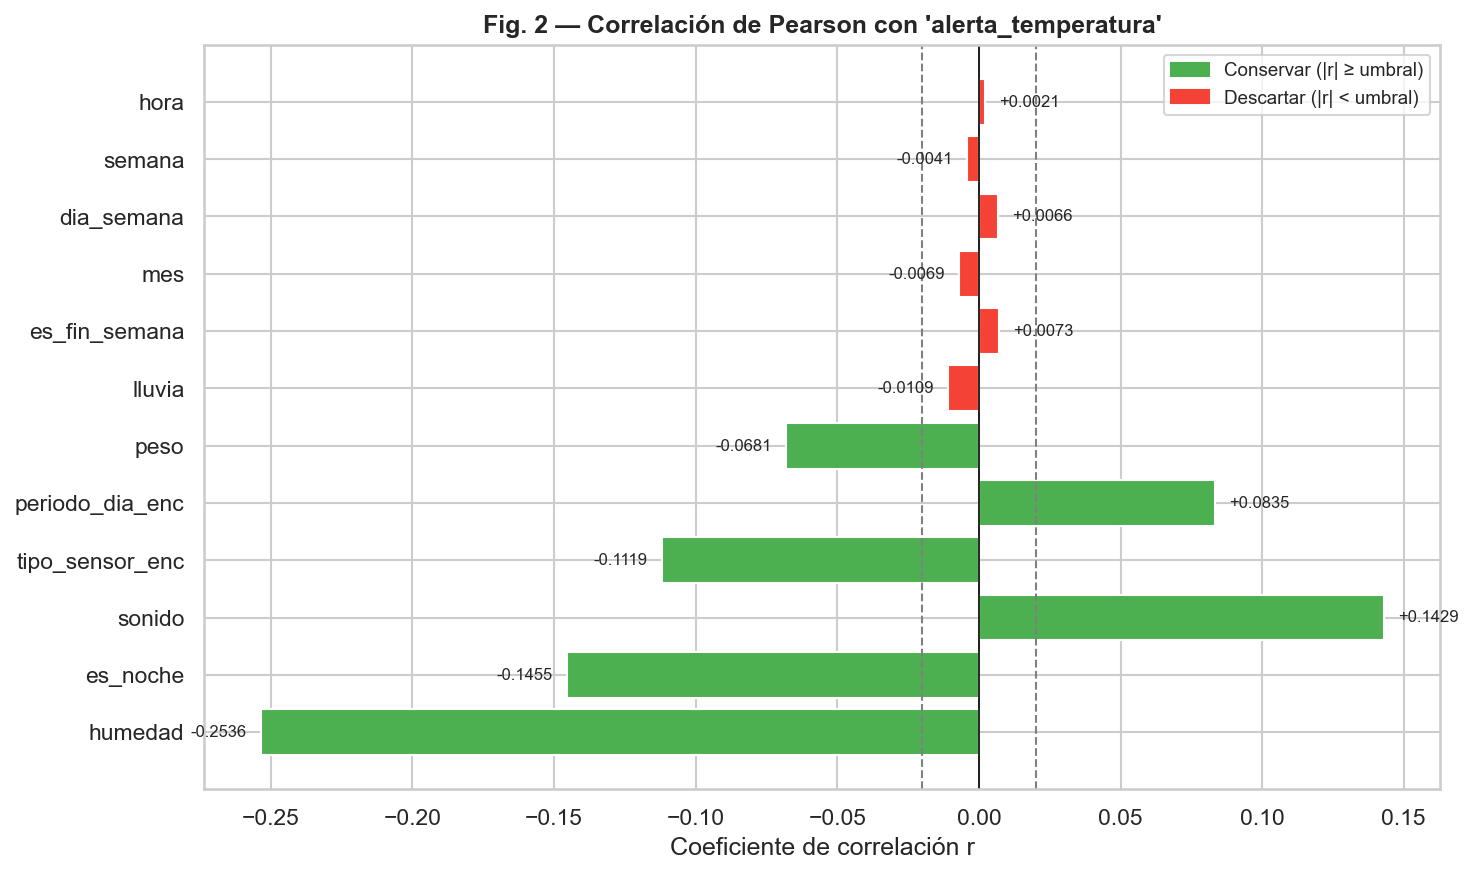
\includegraphics[width=0.9\textwidth]{figures/fig2_pearson_target.png}
  \caption{Coeficiente de Pearson de cada feature con \texttt{alerta\_temperatura}.
           Verde = conservar ($|r| \geq 0.02$).}
\end{figure}

\clearpage

\subsection{M\'etodo 2 --- Umbral de Varianza}

Se descartaron features cuasi-constantes con varianza inferior a 0.01. Ninguna feature
fue eliminada por este criterio, confirmando que todas tienen dispersi\'on suficiente
para aportar informaci\'on al modelo.

\begin{figure}[h!]
  \centering
  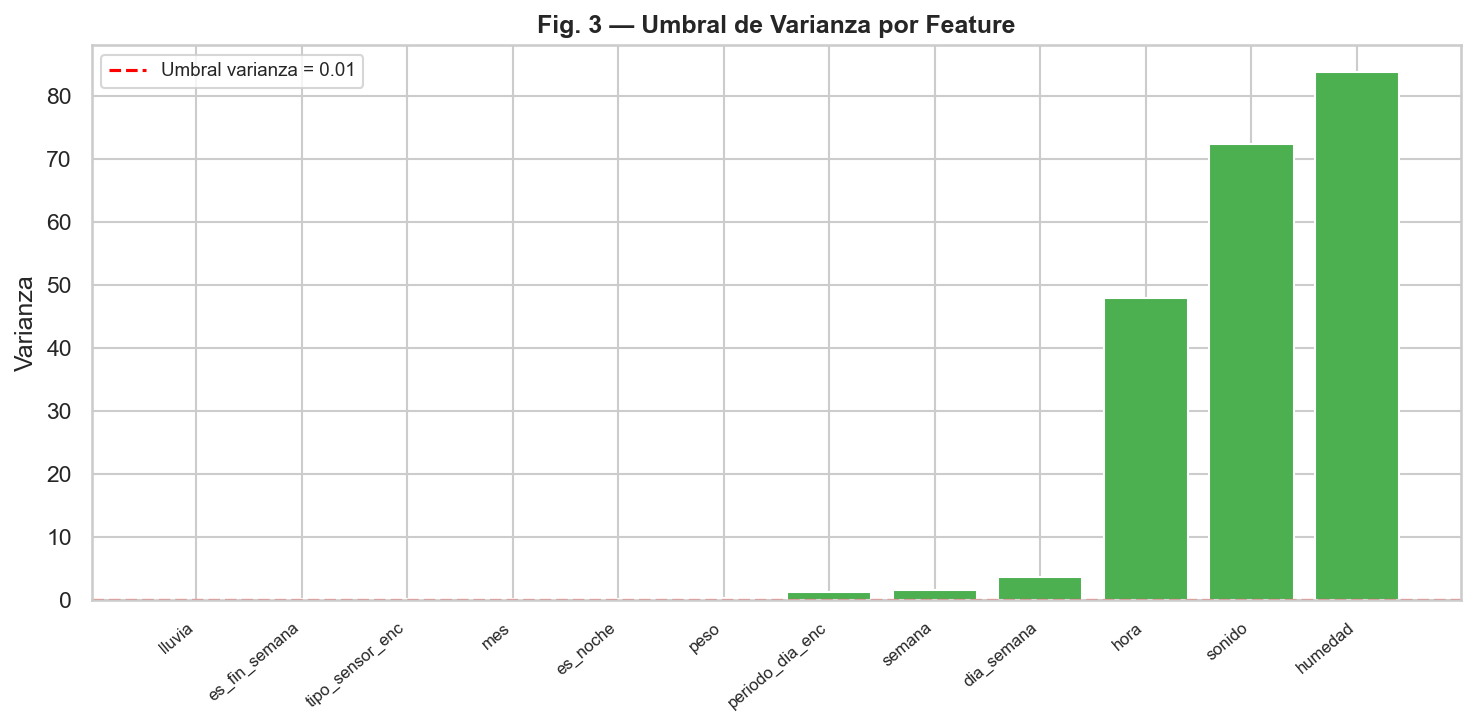
\includegraphics[width=0.9\textwidth]{figures/fig3_varianza.png}
  \caption{Varianza de cada feature. La l\'inea roja marca el umbral de 0.01.}
\end{figure}

\subsection{M\'etodo 3 --- Test Chi-Cuadrado ($\chi^2$)}

El test $\chi^2$ eval\'ua si existe una asociaci\'on estad\'isticamente significativa
entre cada variable discreta o categ\'orica y el target ($H_0$: independencia).
Se rechaza $H_0$ cuando $p < \alpha = 0.05$.

\begin{figure}[h!]
  \centering
  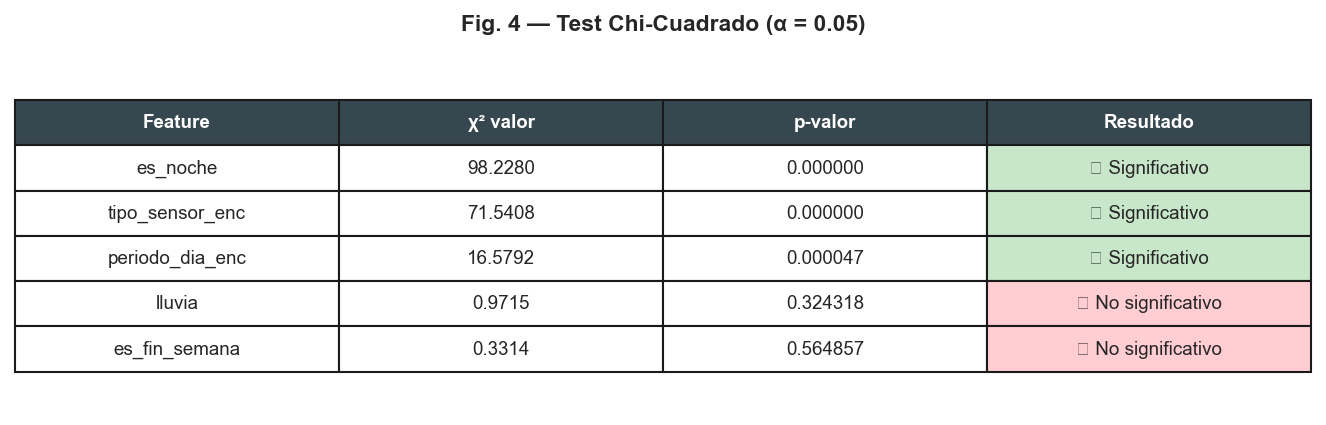
\includegraphics[width=0.85\textwidth]{figures/fig4_chi2_pvalues.png}
  \caption{Resultados del test $\chi^2$. Celdas verdes ($p < 0.05$) indican
           asociaci\'on significativa con el target.}
\end{figure}

\textbf{Descartadas:} \texttt{lluvia} ($p = 0.324$) y \texttt{es\_fin\_semana}
($p = 0.565$). La lluvia no presenta asociaci\'on significativa con alertas de temperatura
porque los eventos de lluvia son independientes del ciclo t\'ermico diario de la colmena.

\subsection{M\'etodo 4 --- Importancia con Random Forest (150 \'arboles)}

Se entren\'o un clasificador Random Forest con 150 \'arboles sobre las features
supervivientes. Las features con importancia Gini inferior a 0.02 se descartaron.

\begin{figure}[h!]
  \centering
  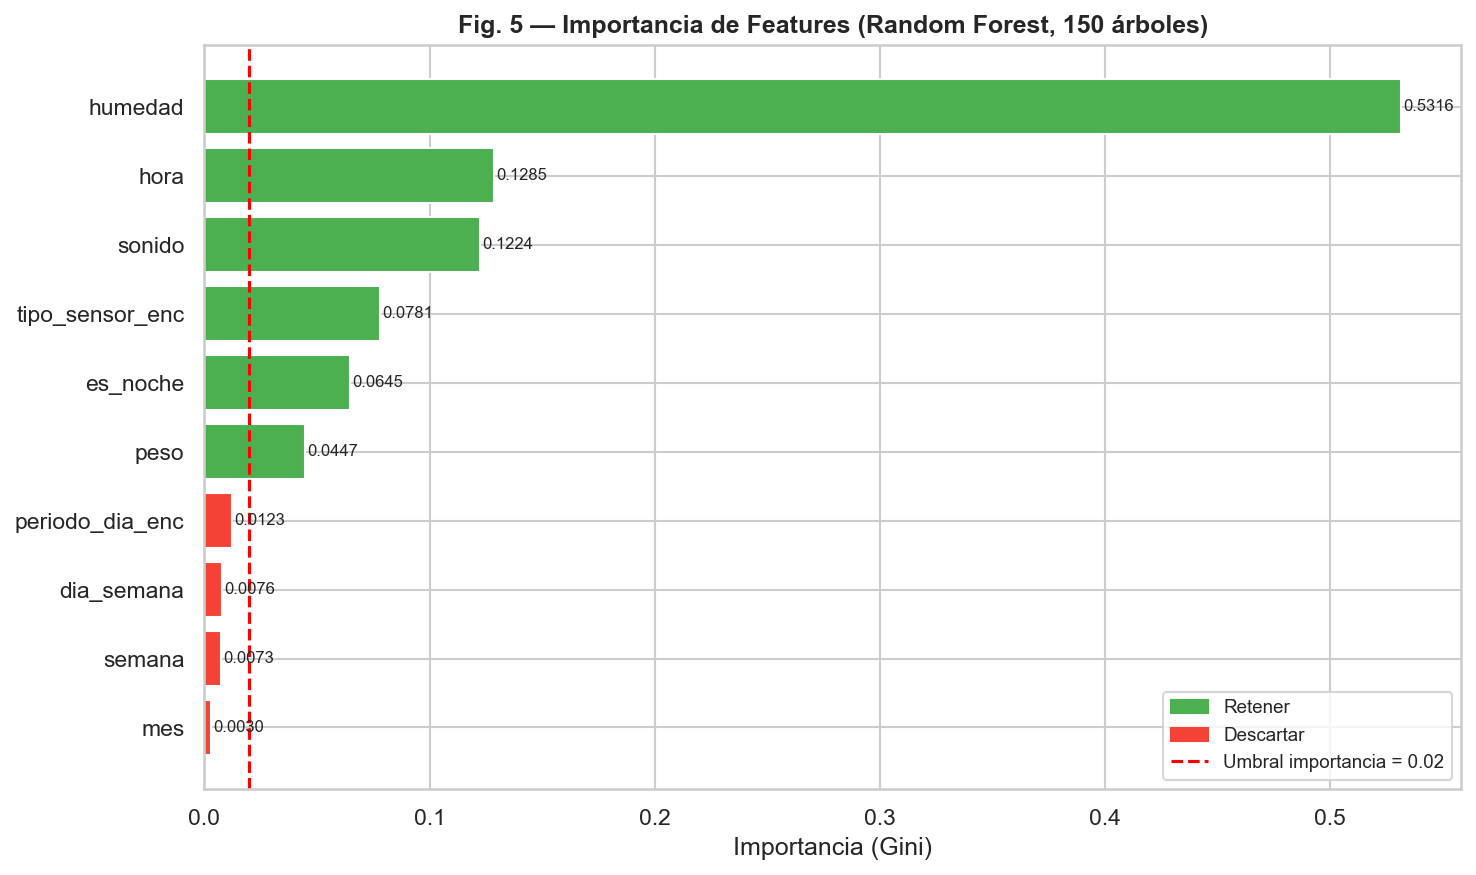
\includegraphics[width=0.9\textwidth]{figures/fig5_rf_importance.png}
  \caption{Importancia Gini por feature. Verde = retenida ($\geq 0.02$),
           rojo = descartada.}
\end{figure}

\clearpage

\subsection{Resumen de Selecci\'on}

\begin{table}[h!]
  \centering
  \caption{Features finales seleccionadas y su justificaci\'on}
  \rowcolors{2}{grisCelda}{white}
  \begin{tabularx}{\textwidth}{lrX}
    \toprule
    \textbf{Feature} & \textbf{Import. RF} & \textbf{Justificaci\'on} \\
    \midrule
    \texttt{humedad}           & 0.5316 & Correlaci\'on inversa fuerte con temperatura ($r \approx -0.8$) \\
    \texttt{hora}              & 0.1285 & La temperatura sigue un ciclo coseno diario con m\'aximo a media tarde \\
    \texttt{sonido}            & 0.1224 & Las abejas \textit{fanners} incrementan la actividad sonora bajo estr\'es t\'ermico \\
    \texttt{tipo\_sensor\_enc} & 0.0781 & Los sensores Multisensor operan en colmenas con distintos microclimas \\
    \texttt{es\_noche}         & 0.0645 & Proxy binario del ciclo d\'ia/noche; temperatura siempre inferior de noche \\
    \texttt{peso}              & 0.0447 & El enjambre por calor puede producir p\'erdida de peso detectable \\
    \bottomrule
  \end{tabularx}
\end{table}

\begin{table}[h!]
  \centering
  \caption{Resumen de reducci\'on dimensional por m\'etodo}
  \rowcolors{2}{grisCelda}{white}
  \begin{tabular}{lr}
    \toprule
    \textbf{M\'etrica} & \textbf{Valor} \\
    \midrule
    Features candidatas iniciales         & 12 \\
    Descartadas por Pearson ($|r|<0.02$)  & 0  \\
    Descartadas por varianza ($<0.01$)    & 0  \\
    Descartadas por Chi-cuadrado ($p\geq0.05$) & 2 \\
    Descartadas por Random Forest ($<0.02$) & 4 \\
    \textbf{Features conservadas}         & \textbf{6} \\
    \textbf{Reducci\'on dimensional}      & \textbf{50\%} \\
    \bottomrule
  \end{tabular}
\end{table}

\subsection{Dataset Final Optimizado}

El archivo \texttt{data/clean/dataset\_final\_features.csv} contiene 8\,573 filas
$\times$ 7 columnas (\texttt{humedad}, \texttt{hora}, \texttt{sonido},
\texttt{tipo\_sensor\_enc}, \texttt{es\_noche}, \texttt{peso},
\texttt{alerta\_temperatura}) y est\'a listo para ser utilizado directamente en el
entrenamiento de modelos de clasificaci\'on (XGBoost, Random Forest, LSTM).

\newpage

\section{Archivos Entregados}

\begin{table}[h!]
  \centering
  \caption{Repositorio de archivos generados por la pr\'actica}
  \rowcolors{2}{grisCelda}{white}
  \begin{tabularx}{\textwidth}{lX}
    \toprule
    \textbf{Archivo} & \textbf{Descripci\'on} \\
    \midrule
    \texttt{00\_generar\_datos.py}              & Genera el dataset sint\'etico de 8\,769 registros con problemas de calidad intencionales \\
    \texttt{01\_sa\_arquitectura\_dw.md}         & Documento SA: dise\~no del Star Schema, inventario de fuentes y t\'ecnicas de limpieza \\
    \texttt{02\_de\_limpieza\_pipeline.py}       & Pipeline DE de 10 pasos con evidencia cuantitativa antes/despu\'es en cada transformaci\'on \\
    \texttt{03\_au\_seleccion\_caracteristicas.py} & Selecci\'on AU: cuatro m\'etodos estad\'isticos con generaci\'on de 5 figuras PNG \\
    \texttt{data/raw/lecturas\_crudas.csv}       & Dataset crudo, 8\,769 filas $\times$ 13 columnas \\
    \texttt{data/clean/lecturas\_limpias.csv}    & Dataset limpio, 8\,573 filas $\times$ 21 columnas \\
    \texttt{data/clean/dataset\_final\_features.csv} & Dataset AU optimizado, 8\,573 filas $\times$ 7 columnas \\
    \texttt{data/clean/log\_limpieza.txt}        & Log completo del pipeline DE \\
    \texttt{data/clean/log\_seleccion.txt}       & Log completo de la selecci\'on AU \\
    \texttt{figures/fig1\,--\,fig5.png}          & Evidencia visual: heatmap, Pearson, varianza, Chi-cuadrado, Random Forest \\
    \bottomrule
  \end{tabularx}
\end{table}

\vspace{0.5cm}
\begin{center}
  \textbf{Repositorio p\'ublico:}
  \url{https://github.com/MarkG777/Evaluacion_BD}
\end{center}


\end{document}
% ══ FIN ══

% (contenido original en linea eliminado, ahora gestionado en sections/)
\iffalse
% ══════════════════════════════════════════════════════════════
\section{Contexto del Caso de Estudio}
% ══════════════════════════════════════════════════════════════

\textbf{AbejaNet Revival} es una plataforma IoT para monitoreo en tiempo real de colmenas de abejas (\textit{Apis mellifera}). El sistema integra:

\begin{itemize}\setlength{\itemsep}{0pt}
  \item \textbf{Sensores ESP32} instalados en las colmenas: temperatura, humedad, peso, decibelios y lluvia.
  \item \textbf{Backend Node.js/Express} con base de datos PostgreSQL (alojado en Render).
  \item \textbf{Aplicaci\'on m\'ovil} React Native/Expo para visualizaci\'on por el apicultor.
  \item \textbf{Panel web} de administraci\'on para gesti\'on de apiarios, usuarios y alertas.
\end{itemize}

La tabla \texttt{lecturas\_ambientales} de la BD operacional es la fuente principal de datos de esta pr\'actica. Dado que el servidor de Render no est\'a activo en este periodo, se generaron datos sint\'eticos fieles a la simulaci\'on del script original \texttt{backend/generate\_mock\_data.js}.

% ══════════════════════════════════════════════════════════════
\section{SA --- Arquitectura del Data Warehouse}
% ══════════════════════════════════════════════════════════════

\subsection{Esquema en Estrella (Star Schema)}

Se dise\~n\'o un \textbf{Esquema en Estrella} con una tabla de hechos central y cuatro dimensiones:

\begin{table}[h!]
  \centering
  \caption{Tabla de Hechos: \texttt{fact\_lecturas\_ambientales}}
  \rowcolors{2}{grisCelda}{white}
  \begin{tabularx}{\textwidth}{llX}
    \toprule
    \textbf{Columna} & \textbf{Tipo} & \textbf{Descripci\'on} \\
    \midrule
    \texttt{id\_lectura}  & BIGSERIAL PK  & Clave surrogate \\
    \texttt{sk\_sensor}   & INTEGER FK    & $\rightarrow$ \texttt{dim\_sensor} \\
    \texttt{sk\_tiempo}   & INTEGER FK    & $\rightarrow$ \texttt{dim\_tiempo} \\
    \texttt{sk\_colmena}  & INTEGER FK    & $\rightarrow$ \texttt{dim\_colmena} \\
    \texttt{sk\_apiario}  & INTEGER FK    & $\rightarrow$ \texttt{dim\_apiario} \\
    \texttt{temperatura}  & DECIMAL(5,2)  & \textcelsius{} interior de la colmena \\
    \texttt{humedad}      & DECIMAL(5,2)  & \% de humedad relativa \\
    \texttt{peso}         & DECIMAL(6,2)  & kg totales de la colmena \\
    \texttt{sonido}       & DECIMAL(5,2)  & dB de actividad son\'ora \\
    \texttt{lluvia}       & SMALLINT      & 1~=~lluvia, 0~=~sin lluvia \\
    \texttt{alerta\_temp} & SMALLINT      & 1 si temperatura $>$ 35\textcelsius{} \\
    \bottomrule
  \end{tabularx}
\end{table}

\subsection{Inventario de Variables}

\begin{table}[h!]
  \centering
  \caption{Clasificaci\'on de variables por tipo estad\'istico}
  \rowcolors{2}{grisCelda}{white}
  \begin{tabularx}{\textwidth}{llllX}
    \toprule
    \textbf{Variable} & \textbf{Tipo} & \textbf{Escala} & \textbf{Unidad} & \textbf{Rango esperado} \\
    \midrule
    \texttt{temperatura} & Continua    & Raz\'on   & \textcelsius{}  & $[0, 45]$ \\
    \texttt{humedad}     & Continua    & Raz\'on   & \%              & $[40, 95]$ \\
    \texttt{peso}        & Continua    & Raz\'on   & kg              & $[10, 30]$ \\
    \texttt{sonido}      & Continua    & Raz\'on   & dB              & $[40, 80]$ \\
    \texttt{lluvia}      & Discreta    & Nominal   & ---             & $\{0, 1\}$ \\
    \texttt{tipo\_sensor}& Categ\'orica& Nominal   & ---             & Temp/Multisensor \\
    \texttt{hora}        & Discreta    & C\'iclica & h               & $[0, 23]$ \\
    \texttt{dia\_semana} & Discreta    & Ordinal   & ---             & $[0, 6]$ \\
    \texttt{es\_noche}   & Discreta    & Nominal   & ---             & $\{0, 1\}$ \\
    \bottomrule
  \end{tabularx}
\end{table}

\subsection{Fuentes de Datos}

\begin{table}[h!]
  \centering
  \caption{Inventario de fuentes de datos}
  \rowcolors{2}{grisCelda}{white}
  \begin{tabularx}{\textwidth}{llX}
    \toprule
    \textbf{Fuente} & \textbf{Tipo} & \textbf{Descripci\'on} \\
    \midrule
    ESP32 POST \texttt{/api/sensor-data} & Estructurada en tiempo real & Lecturas c/10 min \\
    \texttt{generate\_mock\_data.js} & Sint\'etica & Simulaci\'on 30 d\'ias (Node.js) \\
    \texttt{00\_generar\_datos.py} & Sint\'etica & Dataset para esta pr\'actica (Python) \\
    \texttt{abeja\_net\_v4\_postgres.sql} & Relacional & Esquema + semilla de la BD \\
    \bottomrule
  \end{tabularx}
\end{table}

\subsection{Configuraci\'on PostgreSQL (DW local)}

\begin{lstlisting}[language=SQL, caption=\'Indices de optimizaci\'on para el DW]
CREATE SCHEMA abejanet_dw;
CREATE INDEX idx_fact_sk_sensor ON fact_lecturas_ambientales (sk_sensor);
CREATE INDEX idx_fact_sk_tiempo ON fact_lecturas_ambientales (sk_tiempo);
CREATE INDEX idx_dim_tiempo_fecha ON dim_tiempo (fecha_completa);
-- postgresql.conf sugerido:
-- shared_buffers = 512MB | work_mem = 64MB | effective_cache_size = 2GB
\end{lstlisting}

% ══════════════════════════════════════════════════════════════
\section{DE --- Reporte del Proceso de Limpieza}
% ══════════════════════════════════════════════════════════════

\subsection{Problemas de Calidad Introducidos}

El script \texttt{00\_generar\_datos.py} genera datos sint\'eticos bas\'andose en la simulaci\'on de sensores ESP32, e introduce intencionalmente los siguientes problemas de calidad:

\begin{table}[h!]
  \centering
  \caption{Problemas de calidad introducidos en el dataset}
  \rowcolors{2}{grisCelda}{white}
  \begin{tabularx}{\textwidth}{lrX}
    \toprule
    \textbf{Tipo de problema} & \textbf{Cantidad} & \textbf{T\'ecnica de limpieza} \\
    \midrule
    Nulos en \texttt{temperatura} & 346 (4\%) & Forward fill por grupo de sensor \\
    Nulos en \texttt{humedad}     & 432 (5\%) & Forward fill por grupo de sensor \\
    Nulos en \texttt{sonido}      & 259 (3\%) & Forward fill por grupo de sensor \\
    Outliers temperatura $>$45\textcelsius{} o $<$0\textcelsius{} & 86 & Invalidar $\rightarrow$ NaN $\rightarrow$ imputar \\
    Outliers humedad $>$100\%     & 69       & Invalidar $\rightarrow$ NaN $\rightarrow$ imputar \\
    Filas duplicadas              & 129 (1.5\%) & \texttt{drop\_duplicates} \\
    Formato incorrecto en lluvia (\texttt{"si"/"no"}) & 351 (4\%) & Mapeo a entero $\{0,1\}$ \\
    Registros hu\'erfanos sin sensor\_id & 69 (0.8\%) & Eliminaci\'on \\
    \bottomrule
  \end{tabularx}
\end{table}

\subsection{Resultados del Pipeline (Antes vs.\ Despu\'es)}

\begin{table}[h!]
  \centering
  \caption{Evidencia cuantitativa del pipeline de limpieza}
  \rowcolors{2}{grisCelda}{white}
  \begin{tabularx}{\textwidth}{llrrr}
    \toprule
    \textbf{Paso} & \textbf{T\'ecnica} & \textbf{Antes} & \textbf{Despu\'es} & $\Delta$ \\
    \midrule
    0 & Carga del dataset crudo & 8\,769 & 8\,769 & --- \\
    1 & Correcci\'on de tipos y formatos & 8\,769 & 8\,769 & 0 \\
    2 & Eliminaci\'on de duplicados & 8\,769 & 8\,641 & $-128$ \\
    3 & Eliminaci\'on de hu\'erfanos & 8\,641 & 8\,573 & $-68$ \\
    4 & Invalidaci\'on de outliers & 8\,573 & 8\,573 & $+143$ nulos \\
    5 & Imputaci\'on ffill+bfill & --- & --- & $-1\,164$ nulos \\
    6 & Enriquecimiento temporal & 13 cols & 21 cols & $+8$ features \\
    \midrule
    \multicolumn{2}{l}{\textbf{Total registros removidos}} & \multicolumn{2}{r}{196 (2.24\%)} & --- \\
    \bottomrule
  \end{tabularx}
\end{table}

\subsection{Estad\'isticas Post-limpieza (Paso 7 --- Validaci\'on Final)}

\begin{lstlisting}[caption=Salida real del script 02\_de\_limpieza\_pipeline.py]
         temperatura   humedad      peso    sonido
count       8573.000  8573.000  5710.000  8573.000
mean          27.195    61.955    15.910    57.679
std            5.104     9.157     0.737     8.509
min            0.040    44.270    14.440    44.000
max           35.940    79.580    17.380    70.000

Validaciones de rango superadas: temperatura [0,45] OK | humedad [0,100] OK | lluvia {0,1} OK
Dataset limpio: 8573 filas x 21 columnas
\end{lstlisting}

% ══════════════════════════════════════════════════════════════
\section{AU --- Selecci\'on de Caracter\'isticas Avanzada}
% ══════════════════════════════════════════════════════════════

\textbf{Variable objetivo:} \texttt{alerta\_temperatura} = 1 si temperatura $>$ 35\textcelsius{}

\textit{Justificaci\'on:} Owens (1971) y Seeley (1985) documentan que por encima de 35\textcelsius{} las abejas de ventilaci\'on (\textit{fanners}) se activan masivamente, correlacionando con incremento de sonido, descenso de humedad y potencial p\'erdida de peso por enjambre.

Distribuci\'on: 8\,364 negativos (97.6\%) --- 209 positivos (2.4\%).

\subsection{M\'etodo 1 --- Correlaci\'on de Pearson}

Se midi\'o la relaci\'on lineal de cada feature con \texttt{alerta\_temperatura}. Umbral de corte: $|r| \geq 0.02$.

\begin{figure}[h!]
  \centering
  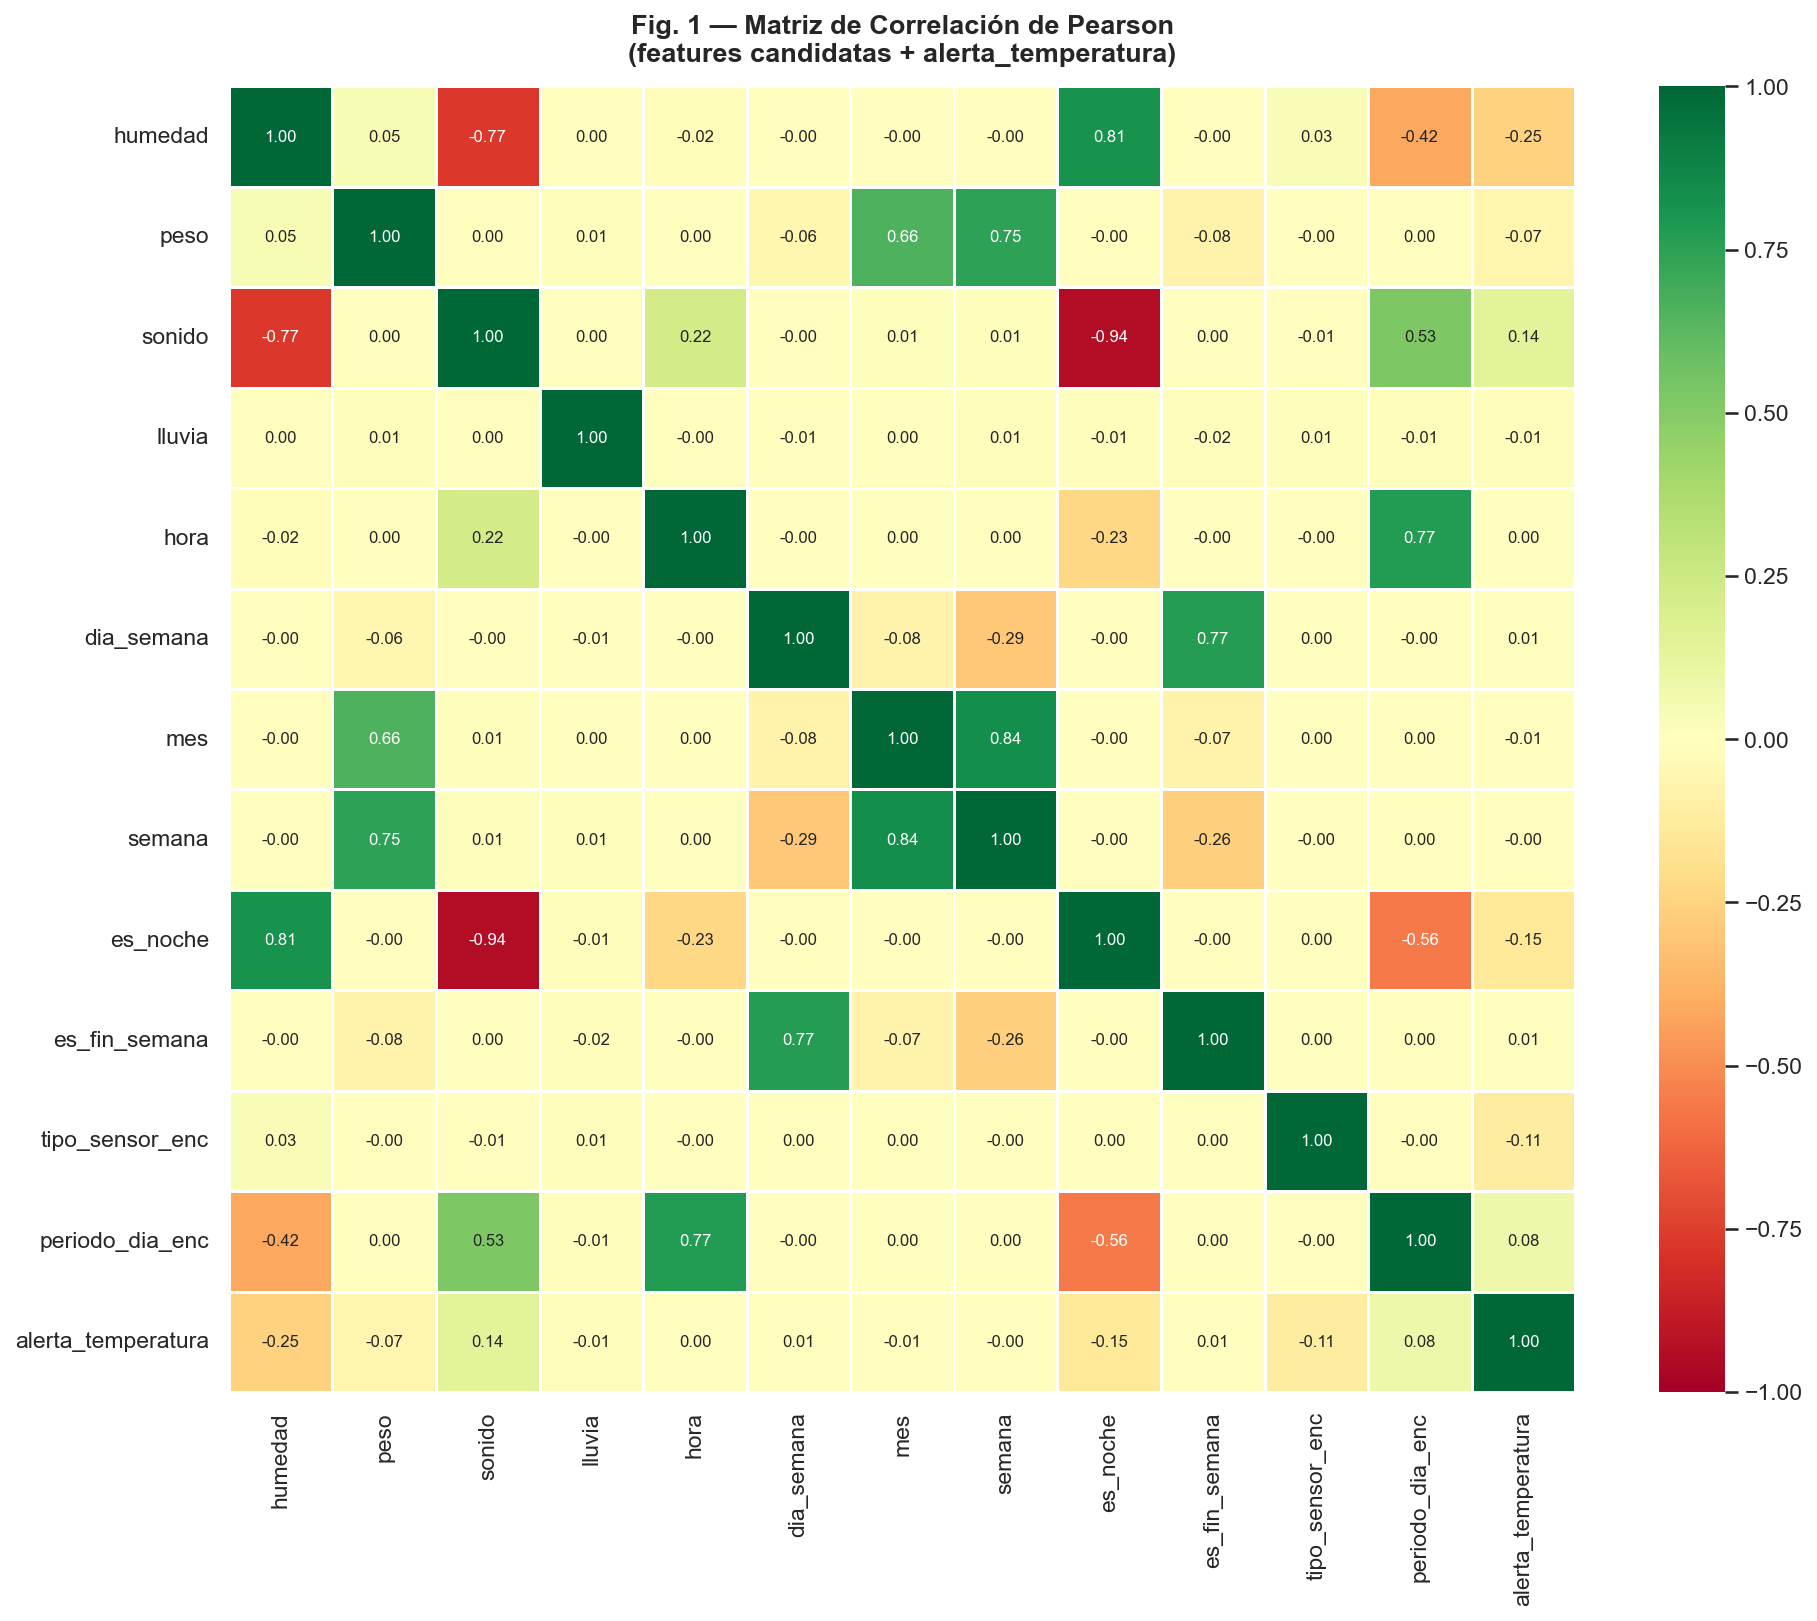
\includegraphics[width=\textwidth]{figures/fig1_heatmap_correlacion.png}
  \caption{Matriz de correlaci\'on de Pearson completa (features candidatas + target)}
\end{figure}

\begin{figure}[h!]
  \centering
  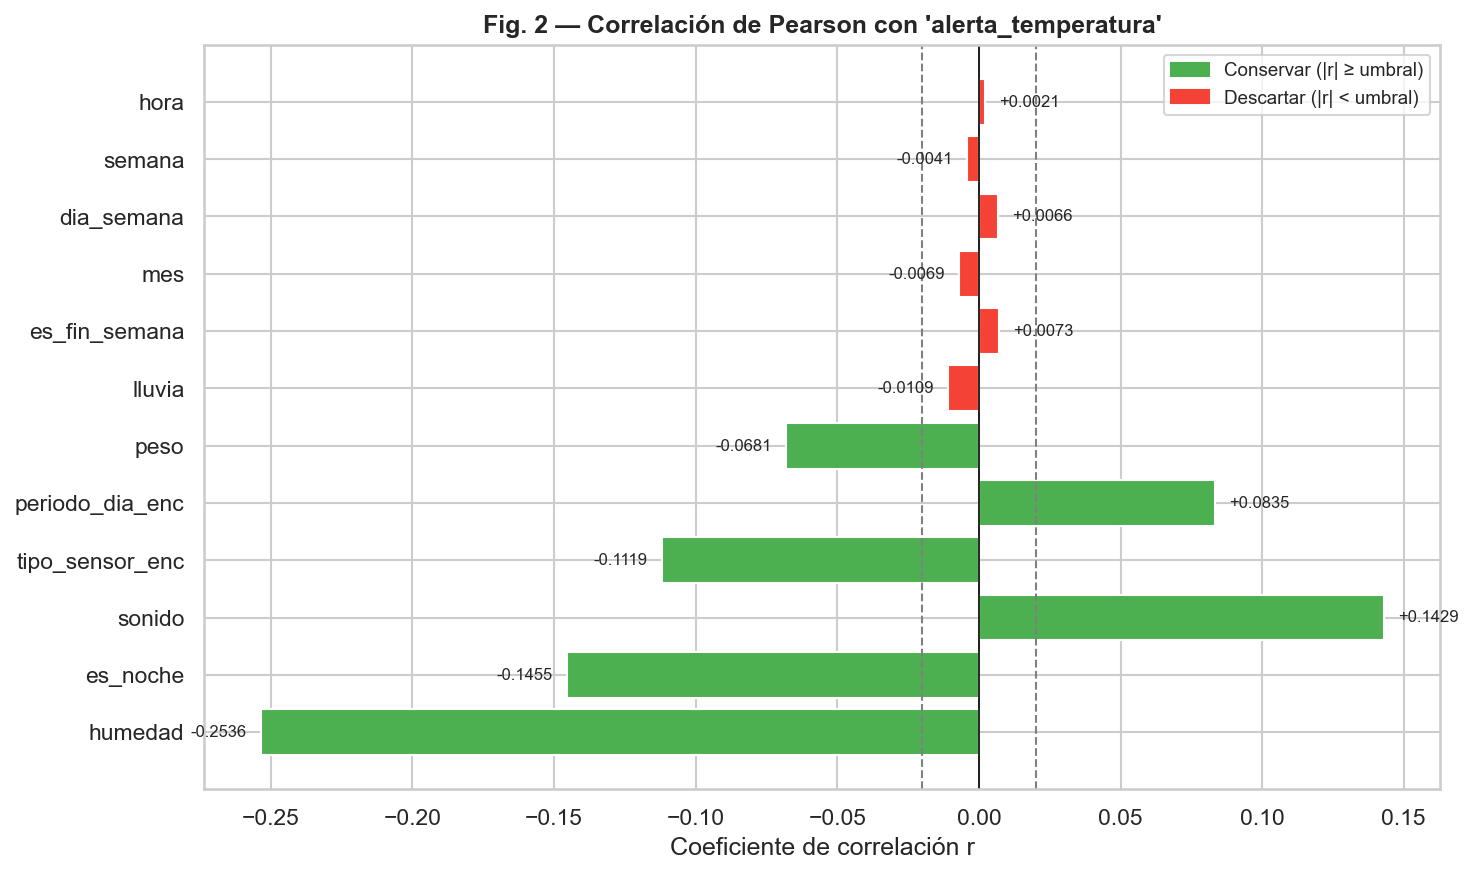
\includegraphics[width=0.9\textwidth]{figures/fig2_pearson_target.png}
  \caption{Correlaci\'on de Pearson de cada feature con \texttt{alerta\_temperatura}}
\end{figure}

Resultado: ninguna feature fue descartada por este m\'etodo --- todas tienen $|r| \geq 0.02$ con el target.

\subsection{M\'etodo 2 --- Umbral de Varianza}

Se descartaron features cuasi-constantes con varianza $< 0.01$.

\begin{figure}[h!]
  \centering
  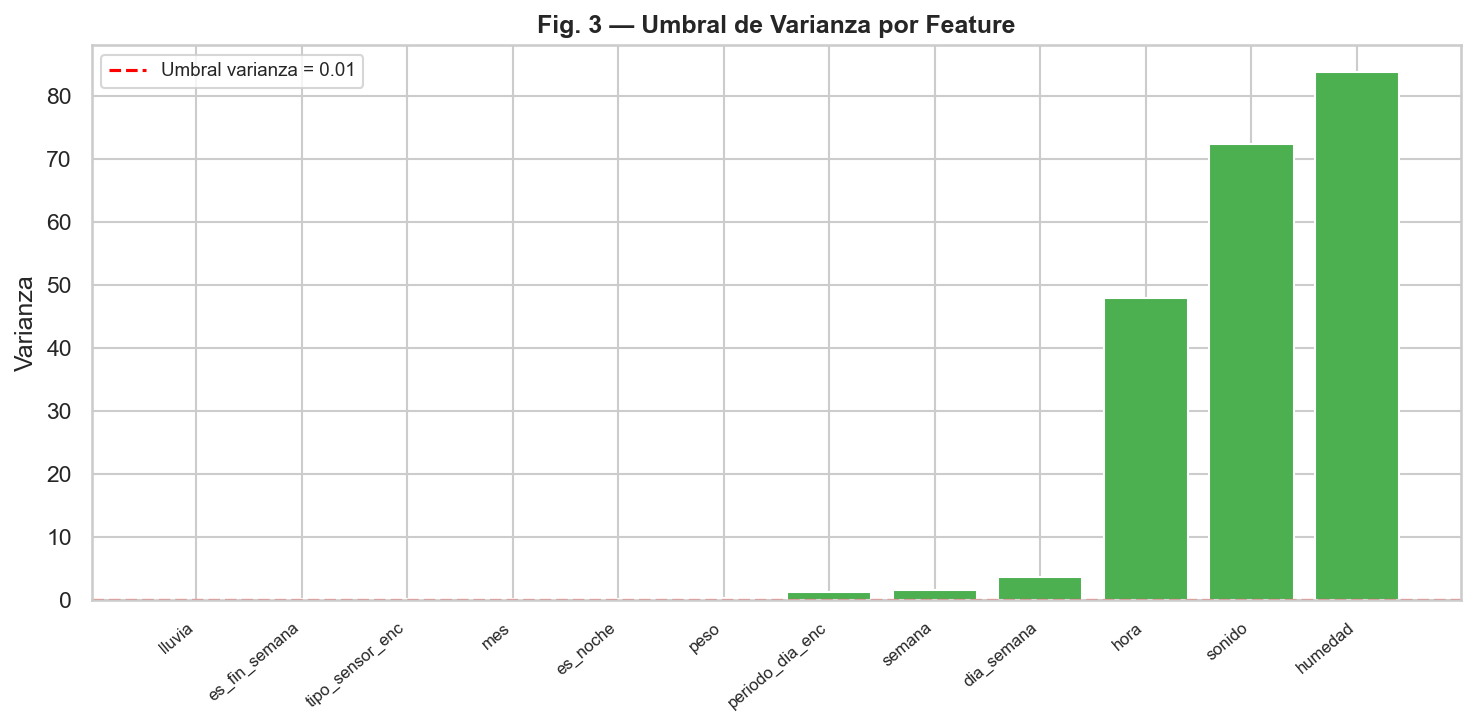
\includegraphics[width=0.9\textwidth]{figures/fig3_varianza.png}
  \caption{Varianza de cada feature. L\'inea roja = umbral de 0.01}
\end{figure}

Resultado: ninguna feature descartada --- todas presentan varianza suficiente.

\subsection{M\'etodo 3 --- Chi-Cuadrado ($\chi^2$)}

Se evalu\'o la asociaci\'on estad\'istica de las variables discretas y categ\'oricas con el target ($\alpha = 0.05$).

\begin{figure}[h!]
  \centering
  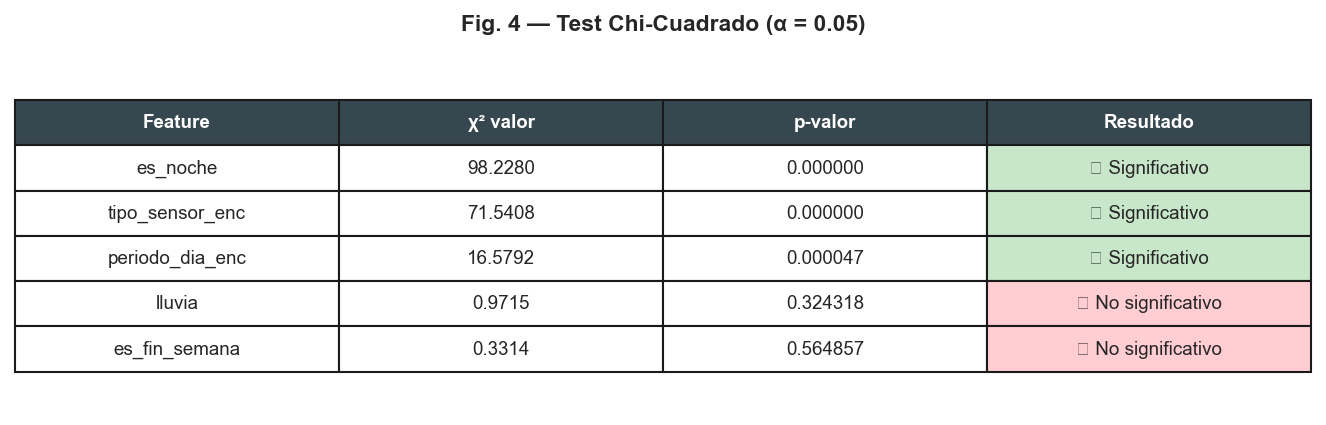
\includegraphics[width=0.85\textwidth]{figures/fig4_chi2_pvalues.png}
  \caption{Resultados del test $\chi^2$. Verde = significativo ($p < 0.05$), rojo = no significativo}
\end{figure}

\textbf{Descartadas:} \texttt{lluvia} ($p = 0.324$) y \texttt{es\_fin\_semana} ($p = 0.565$) --- no existe asociaci\'on estad\'isticamente significativa con el target.

\subsection{M\'etodo 4 --- Importancia con Random Forest}

Se entren\'o un Random Forest con 150 \'arboles sobre las features supervivientes. Umbral de corte: importancia $\geq 0.02$.

\begin{figure}[h!]
  \centering
  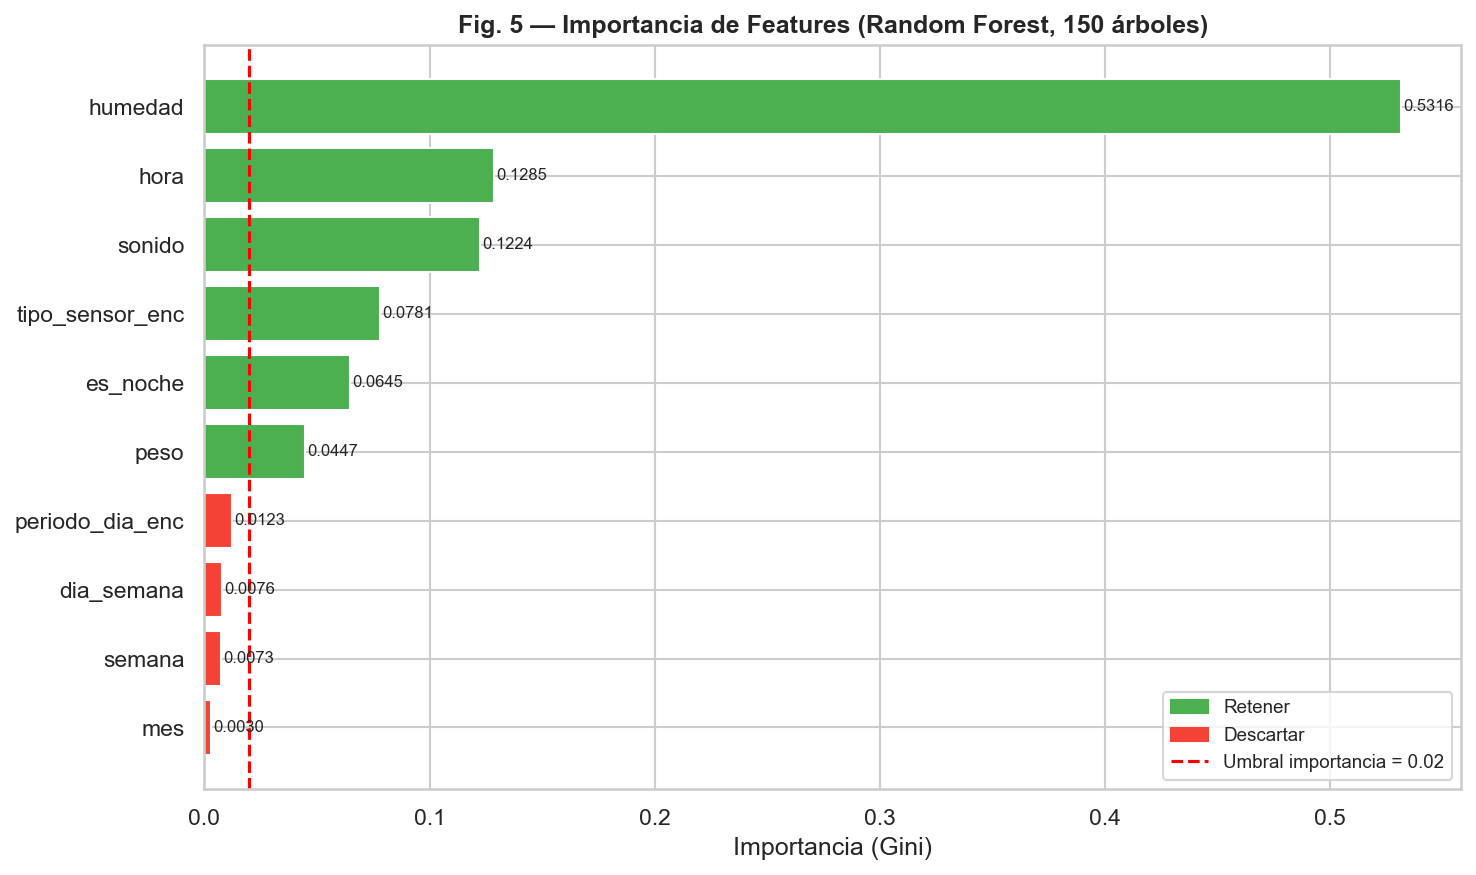
\includegraphics[width=0.9\textwidth]{figures/fig5_rf_importance.png}
  \caption{Importancia (Gini) de features. Verde = retenida, rojo = descartada}
\end{figure}

\subsection{Resumen de Selecci\'on}

\begin{table}[h!]
  \centering
  \caption{Features finales seleccionadas para el modelo}
  \rowcolors{2}{grisCelda}{white}
  \begin{tabularx}{\textwidth}{lrX}
    \toprule
    \textbf{Feature} & \textbf{Import. RF} & \textbf{Justificaci\'on} \\
    \midrule
    \texttt{humedad}        & 0.5316 & Correlaci\'on inversa fuerte con temperatura \\
    \texttt{hora}           & 0.1285 & Temperatura sigue ciclo coseno diario \\
    \texttt{sonido}         & 0.1224 & Actividad de abejas \textit{fanners} bajo estr\'es t\'ermico \\
    \texttt{tipo\_sensor\_enc} & 0.0781 & Multisensores en distintos microclimas \\
    \texttt{es\_noche}      & 0.0645 & Proxy binario del ciclo d\'ia/noche \\
    \texttt{peso}           & 0.0447 & Enjambre por calor $\rightarrow$ p\'erdida de peso \\
    \bottomrule
  \end{tabularx}
\end{table}

\begin{table}[h!]
  \centering
  \caption{Reducci\'on dimensional final}
  \rowcolors{2}{grisCelda}{white}
  \begin{tabular}{lr}
    \toprule
    \textbf{M\'etrica} & \textbf{Valor} \\
    \midrule
    Features candidatas iniciales & 12 \\
    Descartadas por Pearson        & 0  \\
    Descartadas por varianza       & 0  \\
    Descartadas por Chi-cuadrado   & 2  \\
    Descartadas por Random Forest  & 4  \\
    \textbf{Features conservadas}  & \textbf{6} \\
    \textbf{Reducci\'on}           & \textbf{50\%} \\
    \bottomrule
  \end{tabular}
\end{table}

% ══════════════════════════════════════════════════════════════
\section{Archivos Entregados}
% ══════════════════════════════════════════════════════════════

\begin{table}[h!]
  \centering
  \caption{Repositorio de archivos generados}
  \rowcolors{2}{grisCelda}{white}
  \begin{tabularx}{\textwidth}{lX}
    \toprule
    \textbf{Archivo} & \textbf{Descripci\'on} \\
    \midrule
    \texttt{00\_generar\_datos.py} & Generador de dataset sint\'etico \\
    \texttt{01\_sa\_arquitectura\_dw.md} & Documento SA: Star Schema + inventario \\
    \texttt{02\_de\_limpieza\_pipeline.py} & Pipeline DE con evidencia antes/despu\'es \\
    \texttt{03\_au\_seleccion\_caracteristicas.py} & Selecci\'on AU: 4 m\'etodos estad\'isticos \\
    \texttt{data/raw/lecturas\_crudas.csv} & Dataset sucio (8\,769 filas, 13 cols) \\
    \texttt{data/clean/lecturas\_limpias.csv} & Dataset limpio (8\,573 filas, 21 cols) \\
    \texttt{data/clean/dataset\_final\_features.csv} & Dataset AU (8\,573 filas, 7 cols) \\
    \texttt{data/clean/log\_limpieza.txt} & Log completo del pipeline DE \\
    \texttt{data/clean/log\_seleccion.txt} & Log completo de la selecci\'on AU \\
    \texttt{figures/fig1\dots fig5.png} & Evidencia visual (5 gr\'aficas) \\
    \bottomrule
  \end{tabularx}
\end{table}
\fi
